\chapter{APPENDIX: Plots}\label{app:appendixB}
\thispagestyle{empty}
\section{\DuMuX and \MATLAB results comparison}

\begin{figure}
    \centering
    \begin{subfigure}{.5\linewidth}
            \centering
        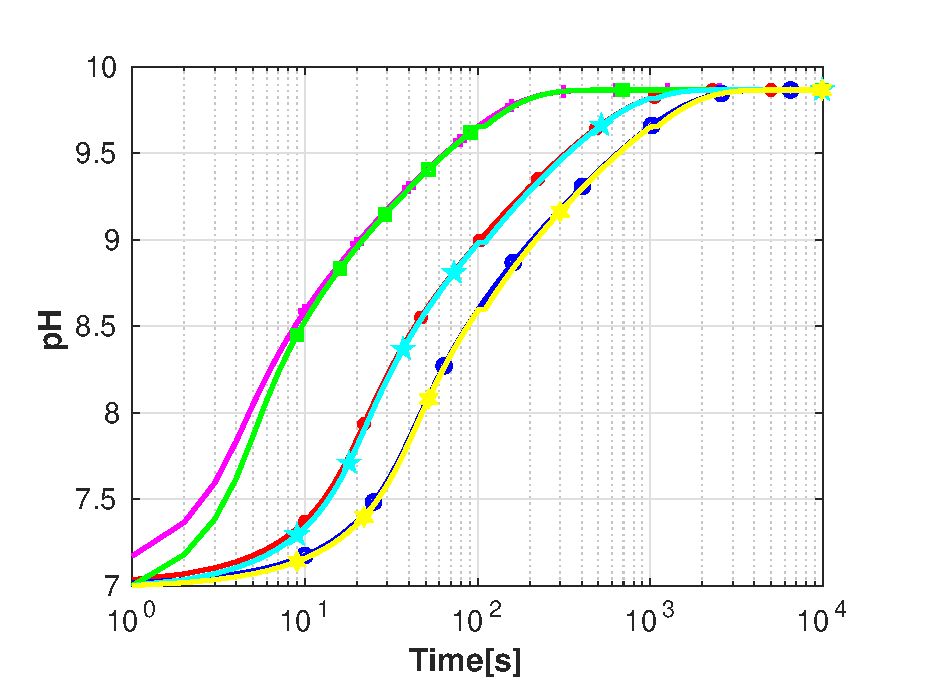
\includegraphics[width=\textwidth]{PICTURES/dvm_pH7_pH.eps}
        \caption{Change in pH}
        \label{fig:dvmpH7pH}
    \end{subfigure}%
        \hfill
    \begin{subfigure}{.5\linewidth}
            \centering
        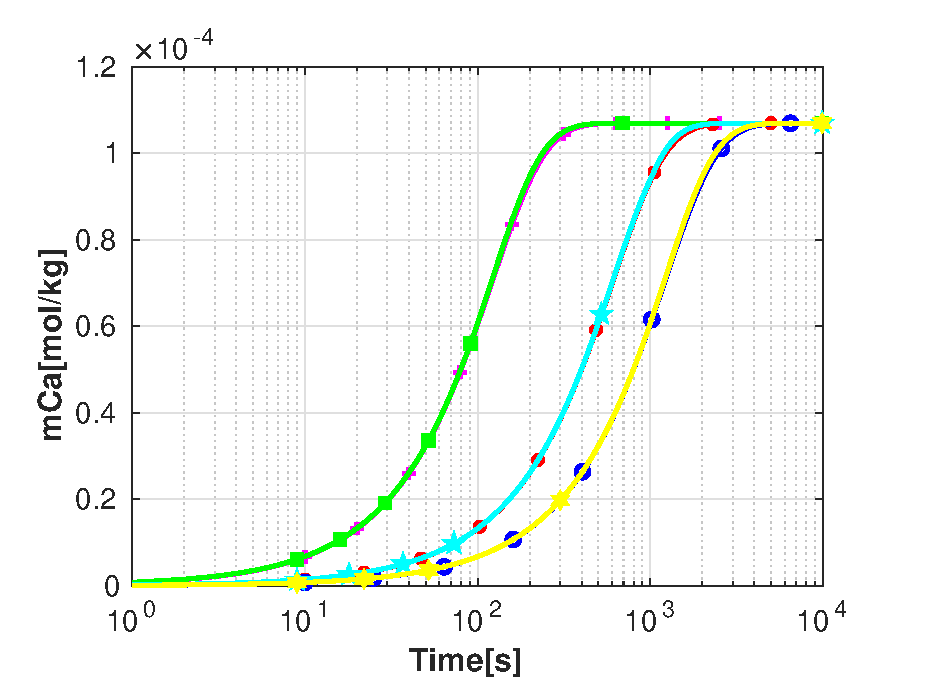
\includegraphics[width=\textwidth]{PICTURES/dvm_pH7_mCa.eps}
        \caption{Change in mCa}
        \label{fig:dvmpH7mCa}
    \end{subfigure}%
    \hfill
    \begin{subfigure}{.5\linewidth}
            \centering
        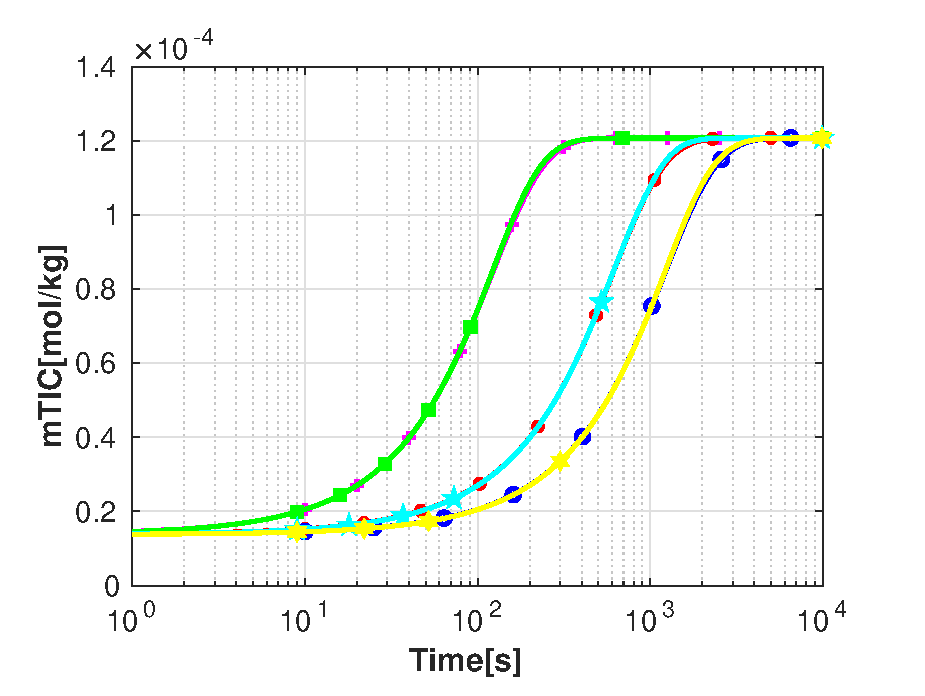
\includegraphics[width=\textwidth]{PICTURES/dvm_pH7_mTIC.eps}
        \caption{Change in mTIC}
        \label{fig:dvmpH7mTIC}
    \end{subfigure}%
    \hfill
    \begin{subfigure}{.5\linewidth}
            \centering
        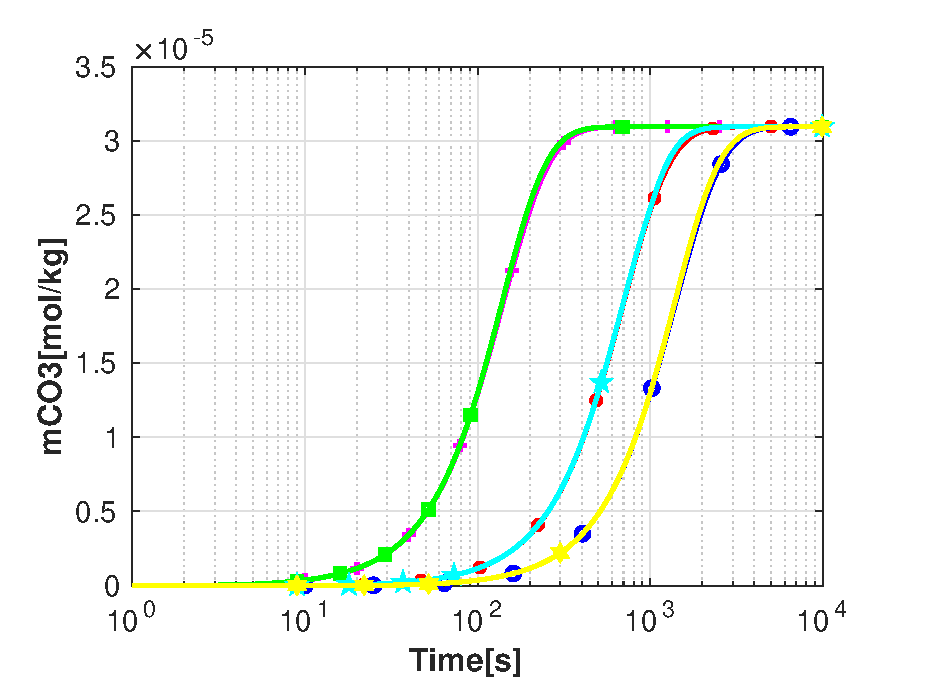
\includegraphics[width=\textwidth]{PICTURES/dvm_pH7_mCO3.eps}
        \caption{Change in mCO3}
        \label{fig:dvmpH7mCO3}
    \end{subfigure}%
    \hfill
    \begin{subfigure}{.5\linewidth}
            \centering
        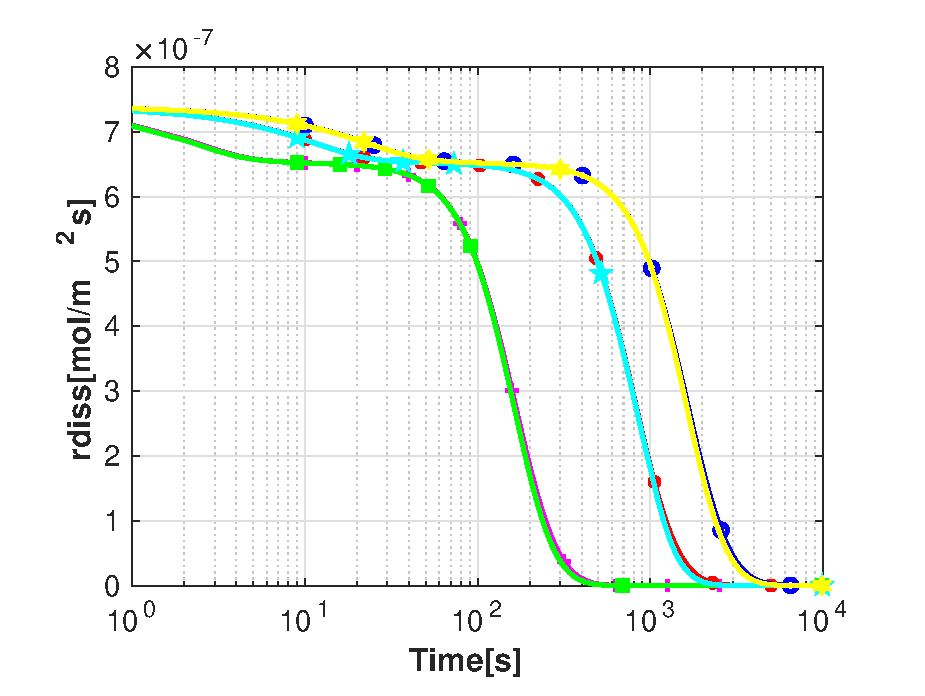
\includegraphics[width=\textwidth]{PICTURES/dvm_pH7_rdiss.eps}
        \caption{Change in rate of dissolution}
        \label{fig:dvmpH7rdiss}
    \end{subfigure}%
   \hfill
   \begin{subfigure}{.5\linewidth}
            \centering
        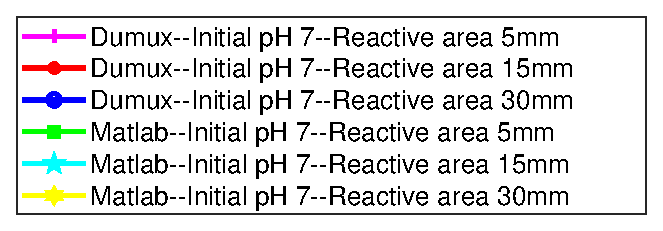
\includegraphics[width=0.85\textwidth]{PICTURES/dvm_pH7_legend.eps}
        \caption{Legend}
        \label{fig:dvmpH7legend}
    \end{subfigure}%
   \caption{Comparison: \DuMuX and \MATLAB results that show the change in pH (\cref{fig:CO2pH}), 
   molality of calcium (\cref{fig:CO2mCa}), molality of total inorganic carbon (\cref{fig:CO2mTIC}), 
   molality of carbonate (\cref{fig:CO2mCO3}) and rate of dissolution of calcite (\cref{fig:CO2rdiss}) 
   in time for initial pH 7.0 in a closed system of 2D volume [15mm $\times$ 5mm]} 
    \label{fig:comparisionDumuxMatlab_pH7.0}
\end{figure}


\begin{figure}
   \centering
   \begin{subfigure}{.5\linewidth}
            \centering
        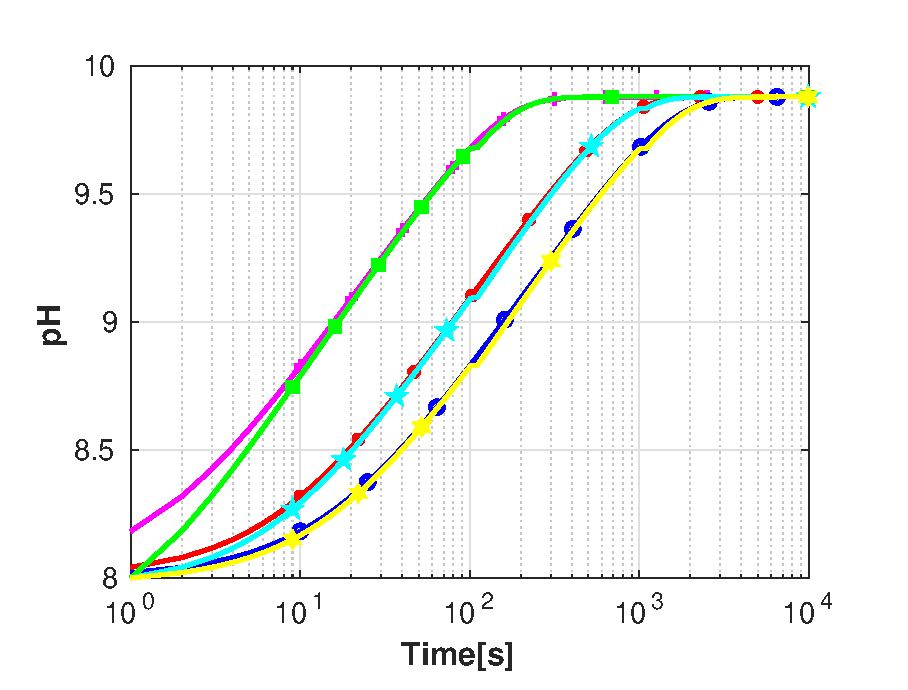
\includegraphics[width=\textwidth]{PICTURES/dvm_pH8_pH.eps}
        \caption{Change in pH}
        \label{fig:dvmpH8pH}
    \end{subfigure}%
        \hfill
    \begin{subfigure}{.5\linewidth}
            \centering
        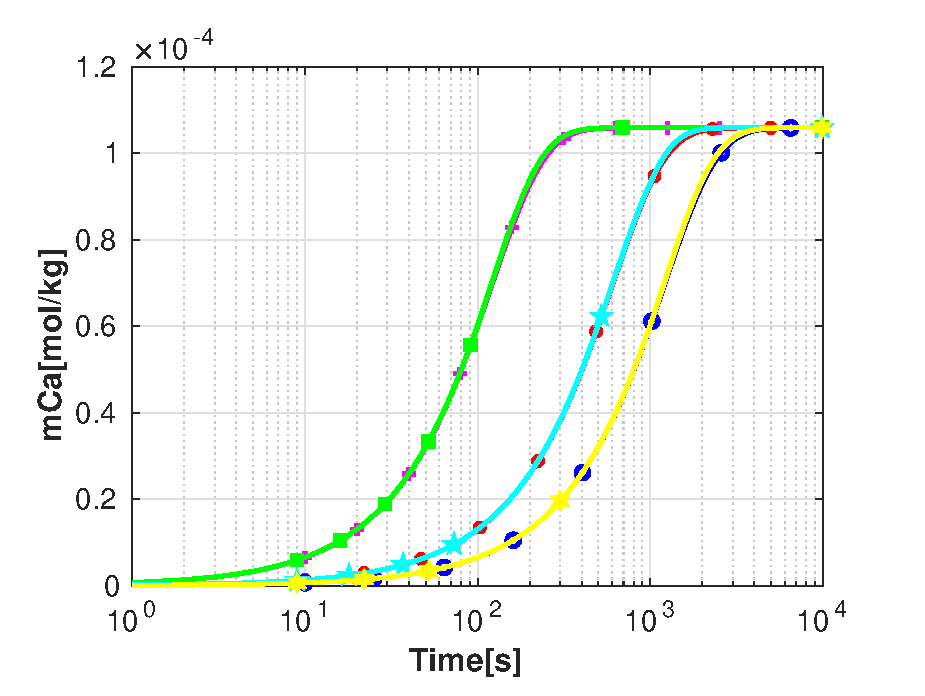
\includegraphics[width=\textwidth]{PICTURES/dvm_pH8_mCa.eps}
        \caption{Change in mCa}
        \label{fig:dvmpH8mCa}
    \end{subfigure}%
    \hfill
    \begin{subfigure}{.5\linewidth}
            \centering
        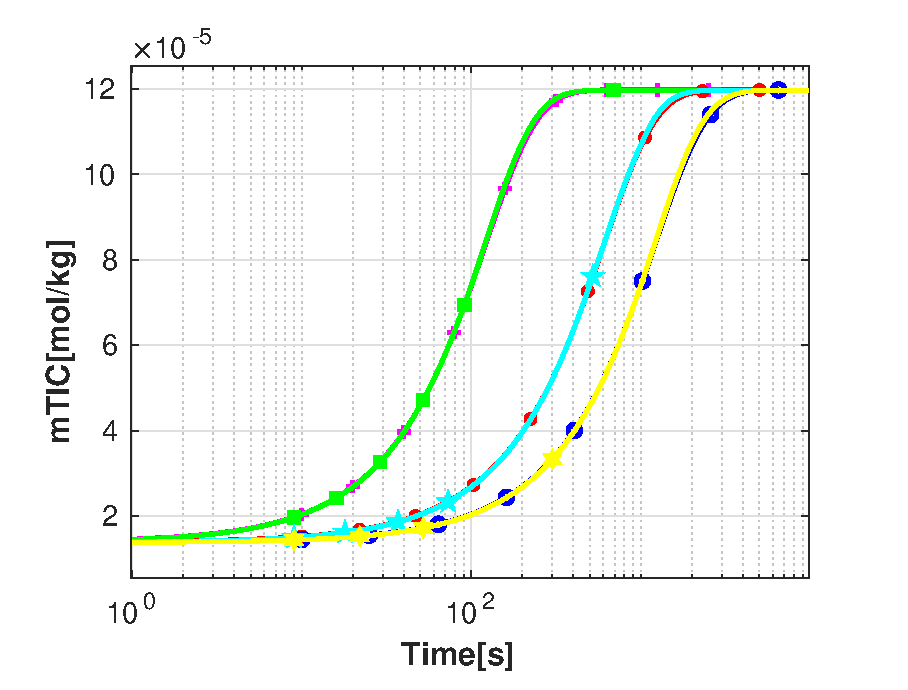
\includegraphics[width=\textwidth]{PICTURES/dvm_pH8_mTIC.eps}
        \caption{Change in mTIC}
        \label{fig:dvmpH8mTIC}
    \end{subfigure}%
    \hfill
    \begin{subfigure}{.5\linewidth}
            \centering
        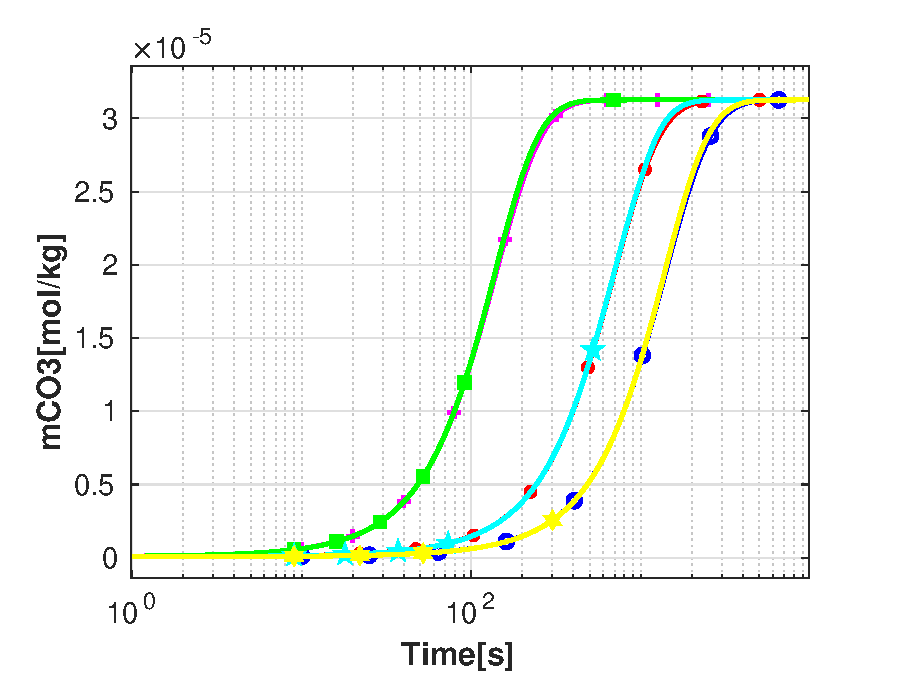
\includegraphics[width=\textwidth]{PICTURES/dvm_pH8_mCO3.eps}
        \caption{Change in mCO3}
        \label{fig:dvmpH8mCO3}
    \end{subfigure}%
    \hfill
    \begin{subfigure}{.5\linewidth}
            \centering
        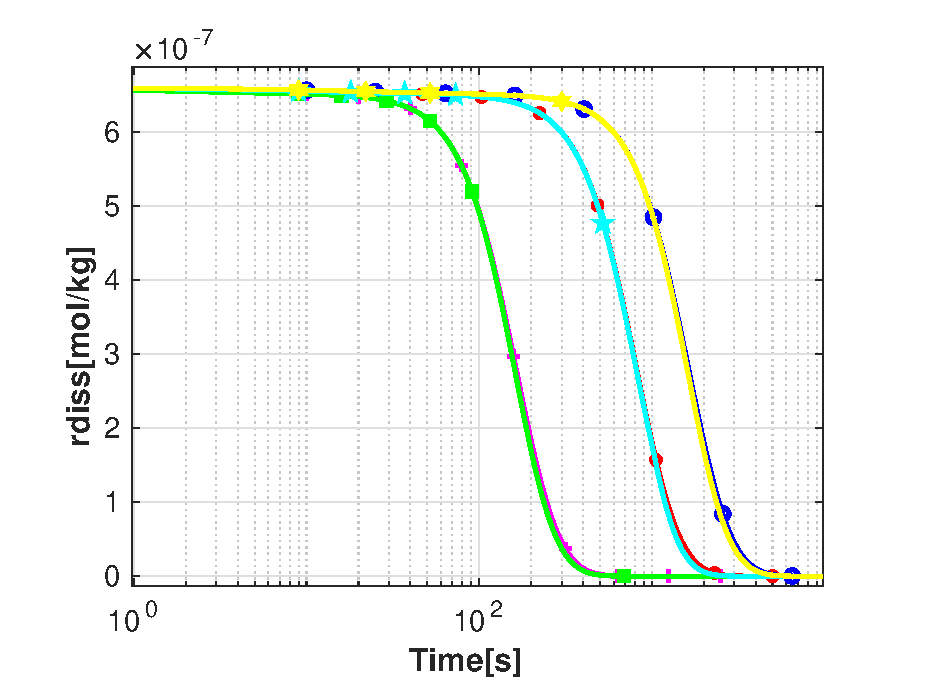
\includegraphics[width=\textwidth]{PICTURES/dvm_pH8_rdiss.eps}
        \caption{Change in rate of dissolution}
        \label{fig:dvmpH8rdiss}
    \end{subfigure}%
   \hfill
   \begin{subfigure}{.5\linewidth}
            \centering
        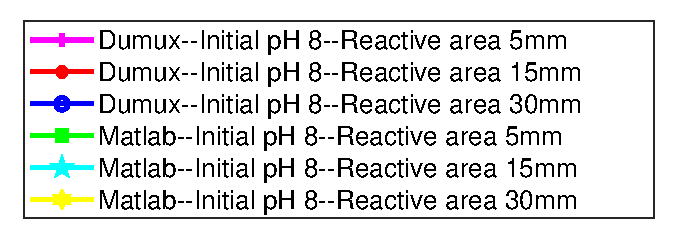
\includegraphics[width=0.85\textwidth]{PICTURES/dvm_pH8_legend.eps}
        \caption{Legend}
        \label{fig:dvmpH8legend}
    \end{subfigure}%
   \caption{Comparison: \DuMuX and \MATLAB results that show the change in pH (\cref{fig:CO2pH}), 
   molality of calcium (\cref{fig:CO2mCa}), molality of total inorganic carbon (\cref{fig:CO2mTIC}), 
   molality of carbonate (\cref{fig:CO2mCO3}) and rate of dissolution of calcite (\cref{fig:CO2rdiss}) 
   in time for initial pH 8.0 in a closed system of 2D volume [15mm $\times$ 5mm]} 
    \label{fig:comparisionDumuxMatlab_pH8.0}
\end{figure}
   
\begin{figure}
   \centering
   \begin{subfigure}{.5\linewidth}
            \centering
        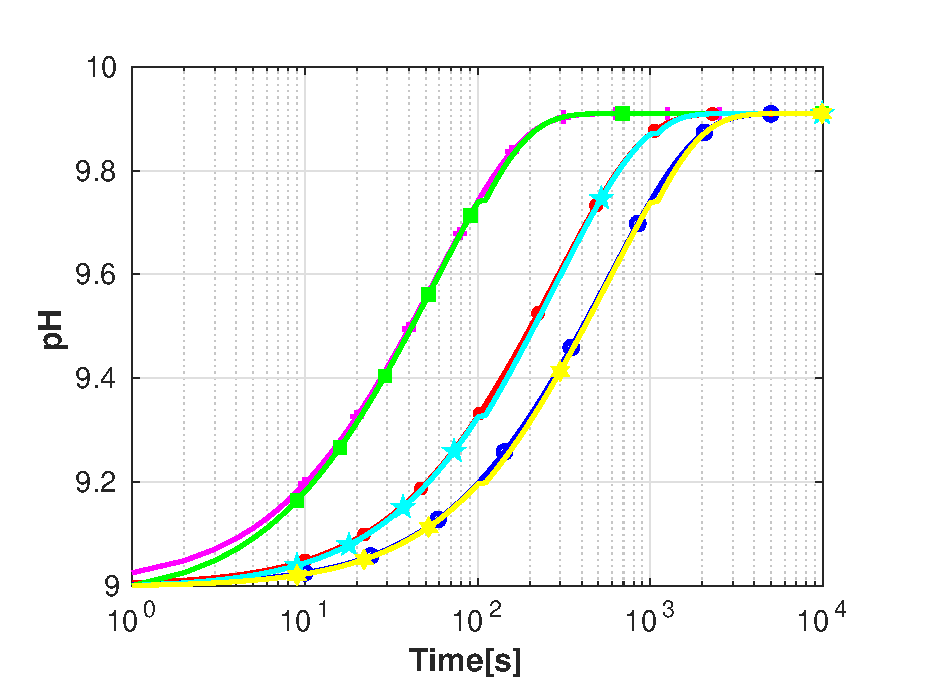
\includegraphics[width=\textwidth]{PICTURES/dvm_pH9_pH.eps}
        \caption{Change in pH}
        \label{fig:dvmpH9pH}
    \end{subfigure}%
        \hfill
    \begin{subfigure}{.5\linewidth}
            \centering
        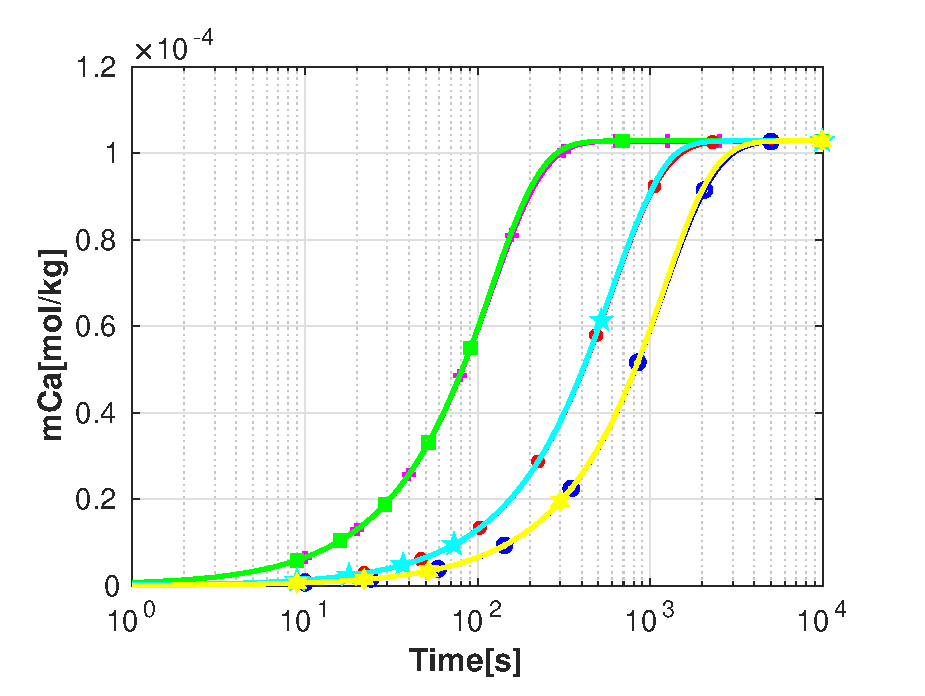
\includegraphics[width=\textwidth]{PICTURES/dvm_pH9_mCa.eps}
        \caption{Change in mCa}
        \label{fig:dvmpH9mCa}
    \end{subfigure}%
    \hfill
    \begin{subfigure}{.5\linewidth}
            \centering
        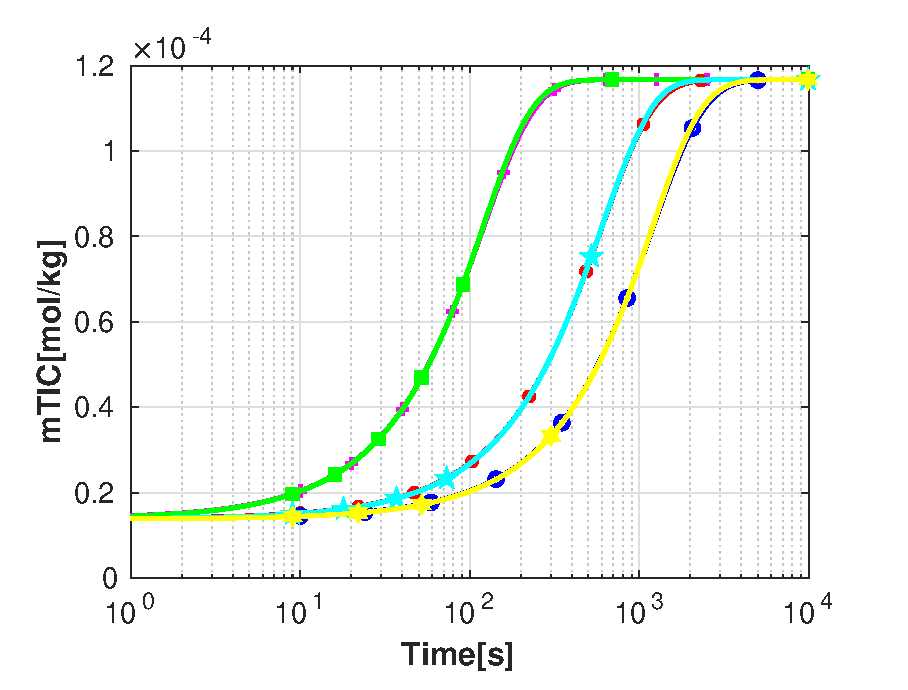
\includegraphics[width=\textwidth]{PICTURES/dvm_pH9_mTIC.eps}
        \caption{Change in mTIC}
        \label{fig:dvmpH9mTIC}
    \end{subfigure}%
    \hfill
    \begin{subfigure}{.5\linewidth}
            \centering
        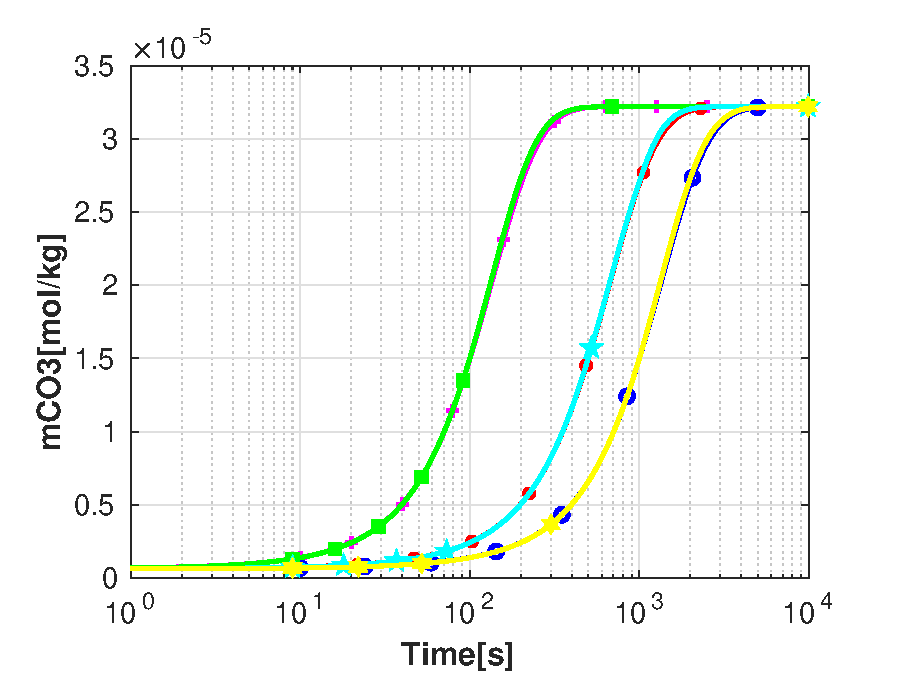
\includegraphics[width=\textwidth]{PICTURES/dvm_pH9_mCO3.eps}
        \caption{Change in mCO3}
        \label{fig:dvmpH9mCO3}
    \end{subfigure}%
    \hfill
    \begin{subfigure}{.5\linewidth}
            \centering
        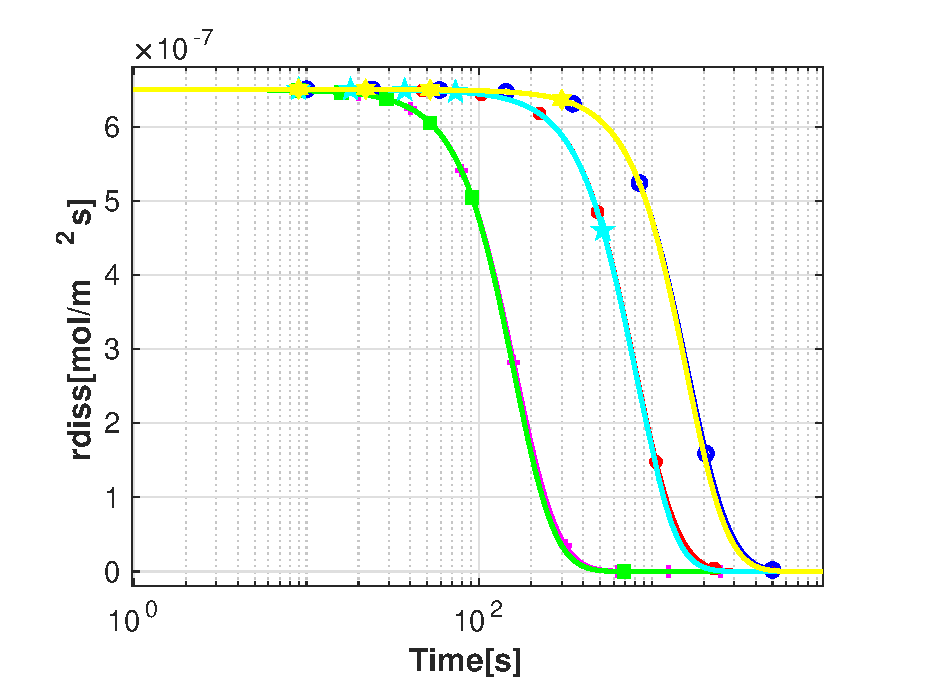
\includegraphics[width=\textwidth]{PICTURES/dvm_pH9_rdiss.eps}
        \caption{Change in rate of dissolution}
        \label{fig:dvmpH9rdiss}
    \end{subfigure}%
    \begin{subfigure}{.5\linewidth}
            \centering
        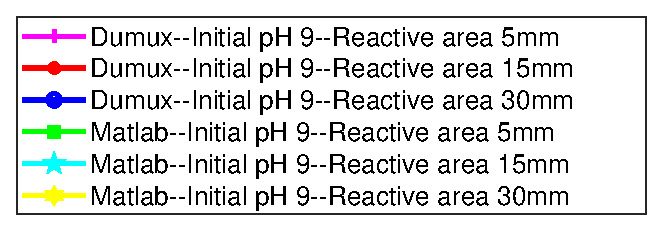
\includegraphics[width=0.85\textwidth]{PICTURES/dvm_pH9_legend.eps}
        \caption{Legend}
        \label{fig:dvmpH9legend}
    \end{subfigure}%
    \caption{Comparison: \DuMuX and \MATLAB results that show the change in pH 
    (\cref{fig:CO2pH}), molality of calcium (\cref{fig:CO2mCa}), molality of total 
    inorganic carbon (\cref{fig:CO2mTIC}), molality of carbonate (\cref{fig:CO2mCO3}) 
    and rate of dissolution of calcite (\cref{fig:CO2rdiss}) in time for initial pH 9.0 in 
    a closed system of 2D volume [15mm $\times$ 5mm]} 
    \label{fig:comparisionDumuxMatlab_pH9.0}
\end{figure}
    
    
\endinput